\documentclass[tikz,border=4pt]{standalone}
\usepackage[T1]{fontenc}
\usepackage{helvet}
\renewcommand{\familydefault}{\sfdefault}
\usetikzlibrary{positioning,arrows.meta,fit,backgrounds,calc}
\definecolor{ill}{HTML}{4C78A8}
\definecolor{ont}{HTML}{E45756}
\definecolor{fus}{HTML}{54A24B}
\definecolor{grey}{HTML}{6B6B6B}
\definecolor{lightgrey}{HTML}{F2F2F2}
\tikzset{
  box/.style={draw=#1, line width=0.8pt, rounded corners=3pt, fill=#1!8, align=center,
              minimum height=10mm, text width=28mm, font=\footnotesize,
              execute at begin node={\hyphenpenalty=10000\exhyphenpenalty=10000}},
  small/.style={draw=#1, line width=0.6pt, rounded corners=2pt, fill=white, align=center,
              minimum height=6mm, text width=30mm, font=\scriptsize,
              execute at begin node={\hyphenpenalty=10000}},
  arr/.style={-{Stealth[length=2.2mm]}, line width=0.8pt, draw=grey},
  lbl/.style={font=\scriptsize\bfseries, text=grey},
}
\begin{document}
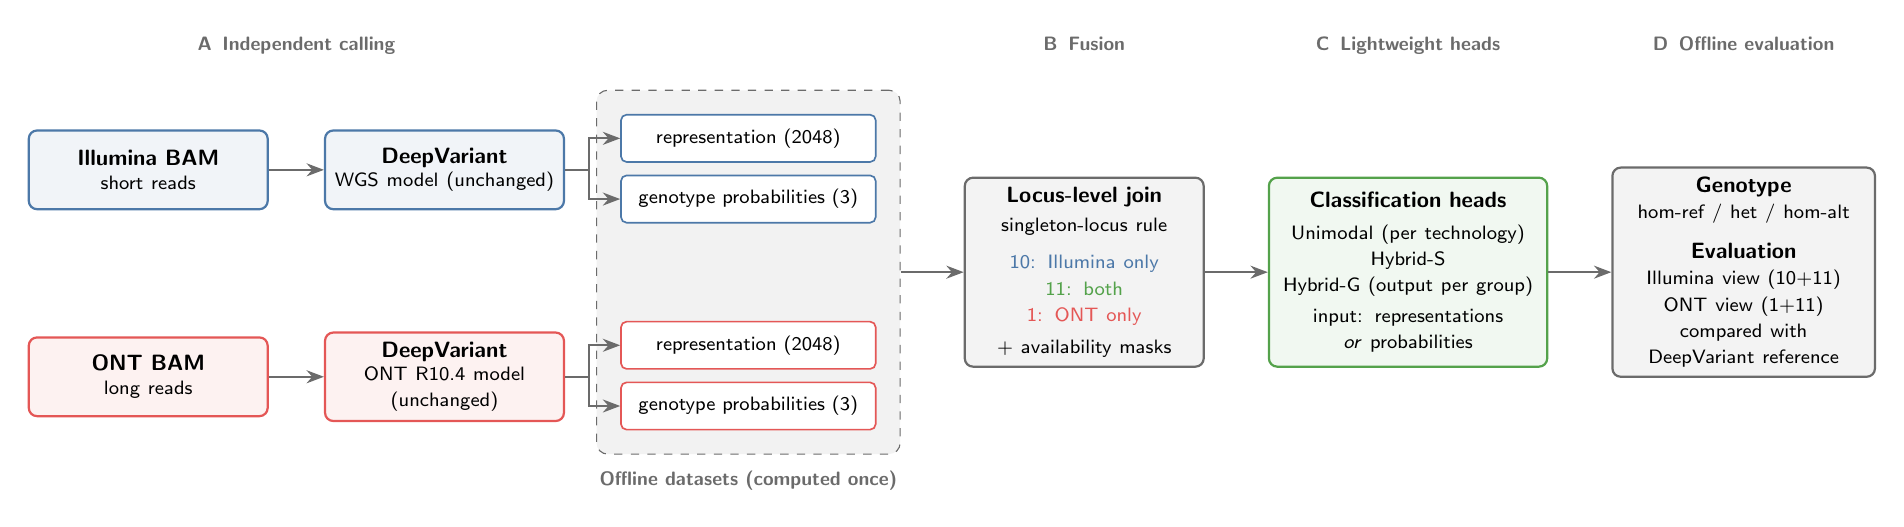
\begin{tikzpicture}[node distance=5mm and 7mm]

% --- Stage 1: inputs and DeepVariant
\node[box=ill] (bamI) {\textbf{Illumina BAM}\\[-1pt]{\scriptsize short reads}};
\node[box=ont, below=16mm of bamI] (bamO) {\textbf{ONT BAM}\\[-1pt]{\scriptsize long reads}};
\node[box=ill, right=of bamI] (dvI) {\textbf{DeepVariant}\\[-1pt]{\scriptsize WGS model (unchanged)}};
\node[box=ont, right=of bamO] (dvO) {\textbf{DeepVariant}\\[-1pt]{\scriptsize ONT R10.4 model (unchanged)}};
\draw[arr] (bamI) -- (dvI);
\draw[arr] (bamO) -- (dvO);

% --- Stage 2: per-candidate outputs
\node[small=ill, right=of dvI, yshift=4mm] (repI) {representation (2048)};
\node[small=ill, below=1.5mm of repI] (prbI) {genotype probabilities (3)};
\node[small=ont, right=of dvO, yshift=4mm] (repO) {representation (2048)};
\node[small=ont, below=1.5mm of repO] (prbO) {genotype probabilities (3)};
\draw[arr] (dvI.east) -- ++(3mm,0) |- (repI.west);
\draw[arr] (dvI.east) -- ++(3mm,0) |- (prbI.west);
\draw[arr] (dvO.east) -- ++(3mm,0) |- (repO.west);
\draw[arr] (dvO.east) -- ++(3mm,0) |- (prbO.west);

% offline dataset band
\begin{scope}[on background layer]
\node[draw=grey, dashed, rounded corners=4pt, fill=lightgrey, inner sep=3mm,
      fit=(repI)(prbI)(repO)(prbO)] (store) {};
\end{scope}
\node[lbl, below=0.8mm of store] {Offline datasets (computed once)};

% --- Stage 3: join
\node[box=grey, right=8mm of store, text width=28mm, minimum height=24mm] (join)
  {\textbf{Locus-level join}\\[1pt]{\scriptsize singleton-locus rule}\\[4pt]
   {\scriptsize\color{ill}10: Illumina only}\\{\scriptsize\color{fus}11: both}\\{\scriptsize\color{ont}1: ONT only}\\[2pt]
   {\scriptsize + availability masks}};
\draw[arr] (store.east) -- (join.west);

% --- Stage 4: heads
\node[box=fus, right=8mm of join, text width=33mm, minimum height=24mm] (heads)
  {\textbf{Classification heads}\\[2pt]
   {\scriptsize Unimodal (per technology)}\\{\scriptsize Hybrid-S}\\{\scriptsize Hybrid-G (output per group)}\\[3pt]
   {\scriptsize input: representations\\ \emph{or} probabilities}};
\draw[arr] (join) -- (heads);

% --- Stage 5: output and evaluation
\node[box=grey, right=8mm of heads, text width=31mm, minimum height=24mm] (eval)
  {\textbf{Genotype}\\{\scriptsize hom-ref / het / hom-alt}\\[5pt]
   \textbf{Evaluation}\\{\scriptsize Illumina view (10+11)}\\{\scriptsize ONT view (1+11)}\\{\scriptsize compared with}\\{\scriptsize DeepVariant reference}};
\draw[arr] (heads) -- (eval);

% stage labels, aligned on one baseline
\coordinate (top) at ($(store.north)+(0,5mm)$);
\node[lbl, anchor=base] at (bamI.north -| {$(bamI)!0.5!(dvI)$}) [yshift=5mm] {};
\node[lbl, anchor=base] at ({$(bamI)!0.5!(dvI)$} |- top) {A\enspace Independent calling};
\node[lbl, anchor=base] at (store.north |- top) {};
\node[lbl, anchor=base] at (join.north |- top) {B\enspace Fusion};
\node[lbl, anchor=base] at (heads.north |- top) {C\enspace Lightweight heads};
\node[lbl, anchor=base] at (eval.north |- top) {D\enspace Offline evaluation};

\end{tikzpicture}
\end{document}
